
    \begin{abstract_online}{Microscopic Structure and Carbon Dioxide Adsorption Properties of 6FDA/BPDA-DAM Polymeric Membrane}{%
        \underline{P. K. Roy}$^{1}$, G. Ayappa$^{2}$, P. K. Maiti$^{1}$}{%
        }{%
        $^1$ Department of Physics, Indian Institute of Science, Bangalore-12, India\newline{}$^2$ Department of Chemical Engineering, Indian Institute of Science, Bangalore-12, India}
    Polymeric membranes are widely accepted as good alternatives for $CO_2$ adsorption from flue gas, as the process is easy to handle and environmentally friendly. Carbon Molecular Sieve (CMS) membranes are obtained via pyrolysis of such polymeric membranes, which also show high solubility, permeability, and selectivity towards $CO_2$ molecules [1]. In the case of 6FDA/BPDA-DAM polymer membrane, the cause of high perm-selectivity towards $CO_2$ is attributed to a rich distribution of ultra-micropores and micropores. To understand the underlying statistics of the pores and their effects on the $CO_2$ adsorption process, an all-atom Dreiding [2] based force-field is prepared to model this polymer. The force-field is parameterized with the help of dihedral scans. A compression-decompression step, followed by repeated annealing steps are performed using molecular dynamics methods, to obtain the optimum density at room temperature and pressure. The glass transition temperature and porosity of the polymer are also calculated, which matched well with the experimental values. The atomistic distribution along the wall of the pores is calculated using an analytical free-volume calculation method [3]. The pore-size distribution is also calculated, which showed a bi-modal distribution. The solubility of the $CO_2$ molecules inside the polymer matrix is calculated using grand canonical Monte Carlo methods, which showed a high affinity towards $CO_2$ molecules. The swelling effects are also studied using a coupled NPT/NVT method. The derived CMS membrane is prepared as a random distribution of pyrrole and pyridine rings [4]. After equilibration, pore-size distribution and $CO_2$ adsorption properties of this CMS membrane are investigated. \begin{center}  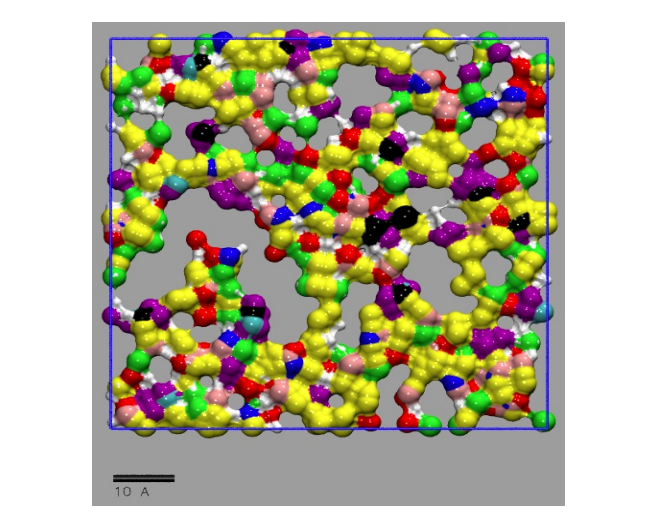
\includegraphics[width=0.5\linewidth]{abstracts/txt/figures/projesh1.png}  \caption{\textbf{Figure 1:} A slice of the equilibrated polymer matrix (XY plane) showing various pores.}  \end{center}  \begin{center}  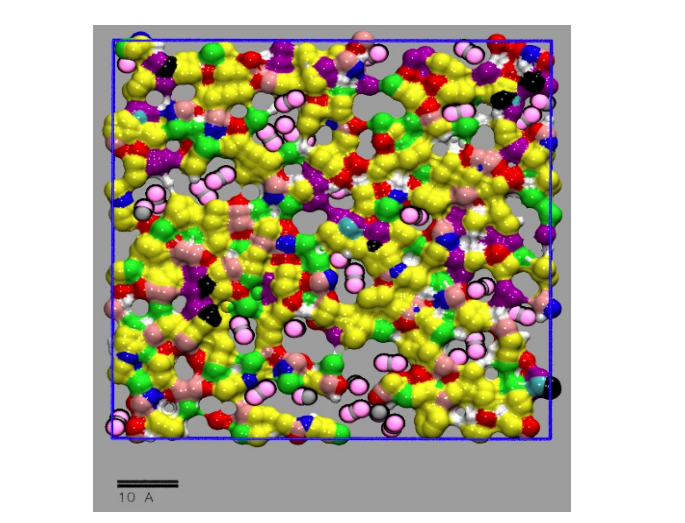
\includegraphics[width=0.5\linewidth]{abstracts/txt/figures/projesh2.png}  \caption{\textbf{Figure 2:} A slice of the equilibrated polymer matrix (XY plane) upon $CO_2$ (Oxygen – Pink, Carbon – Gray ) adsorption and swelling.}  \end{center}  
    
        \textbf{References} \newline{}[1] K. M. Steel, W. J. Koros, Carbon 43 (2005) 1843 – 1856.\newline{}[2] S. L. Mayo, B. D. Olafson, W. A. Goddard, The Journal of Physical Chemistry 94 (1990) 8897–8909. \newline{}[3] G. Zamanakos, 2002. PhD Thesis, California Institute of Technology, Pasadena, California.\newline{}[4] J. S. Adams, A. K. Itta, C. Zhang, G. B. Wenz, O. Sanyal, W. J. Koros, Carbon 141 (2019) 238 – 246 
    \end{abstract_online}
    